% !TeX program = lualatex
% !TeX encoding = utf8
% !TeX spellcheck = uk_UA

\documentclass[tikz,
border=1cm
]{standalone}


\usetikzlibrary{decorations}
\pgfdeclaredecoration{arrows}{draw}{
\state{draw}[width=\pgfdecoratedinputsegmentlength]{%
  \path [every arrow subpath/.try] \pgfextra{%
    \pgfpathmoveto{\pgfpointdecoratedinputsegmentfirst}%
    \pgfpathlineto{\pgfpointdecoratedinputsegmentlast}%
   };
}}
\tikzset{every arrow subpath/.style={-latex, draw, thick}}


\begin{document}


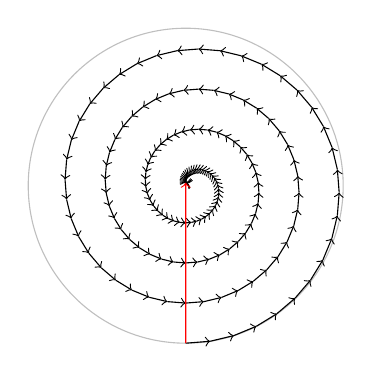
\begin{tikzpicture} % separate paths
\pgfmathsetmacro\N{20}
\pgfmathsetmacro\n{8*\N}
\pgfmathsetmacro\E{2}
\pgfmathsetmacro\k{0.002}
\draw[gray!50] (0,\E) circle (\E);
\coordinate (@) at (0,0);

\foreach \i in {1,...,\n}
{

    \draw[->] (@) -- coordinate[at end] (@) ++ ({(2*\i-1)*pi/2/\N r}:{(pi*\E/\N - \k*\i)});
}

\draw[->, red] (0,0) -- (@);
\end{tikzpicture}



\end{document}


